\renewcommand{\secCol}{White}
\renewcommand{\txtCol}{Sepia}
\pagecolor{CarnationPink}

\addchapter{Ham and Cheese Sandwiches}
{\begin{center}\fontsize{48}{48}\selectfont
\textcolor{RoyalPurple}{\textbf{Ham and Cheese Sandwiches}}
\end{center}}

\begin{center}
\vspace{.25in}
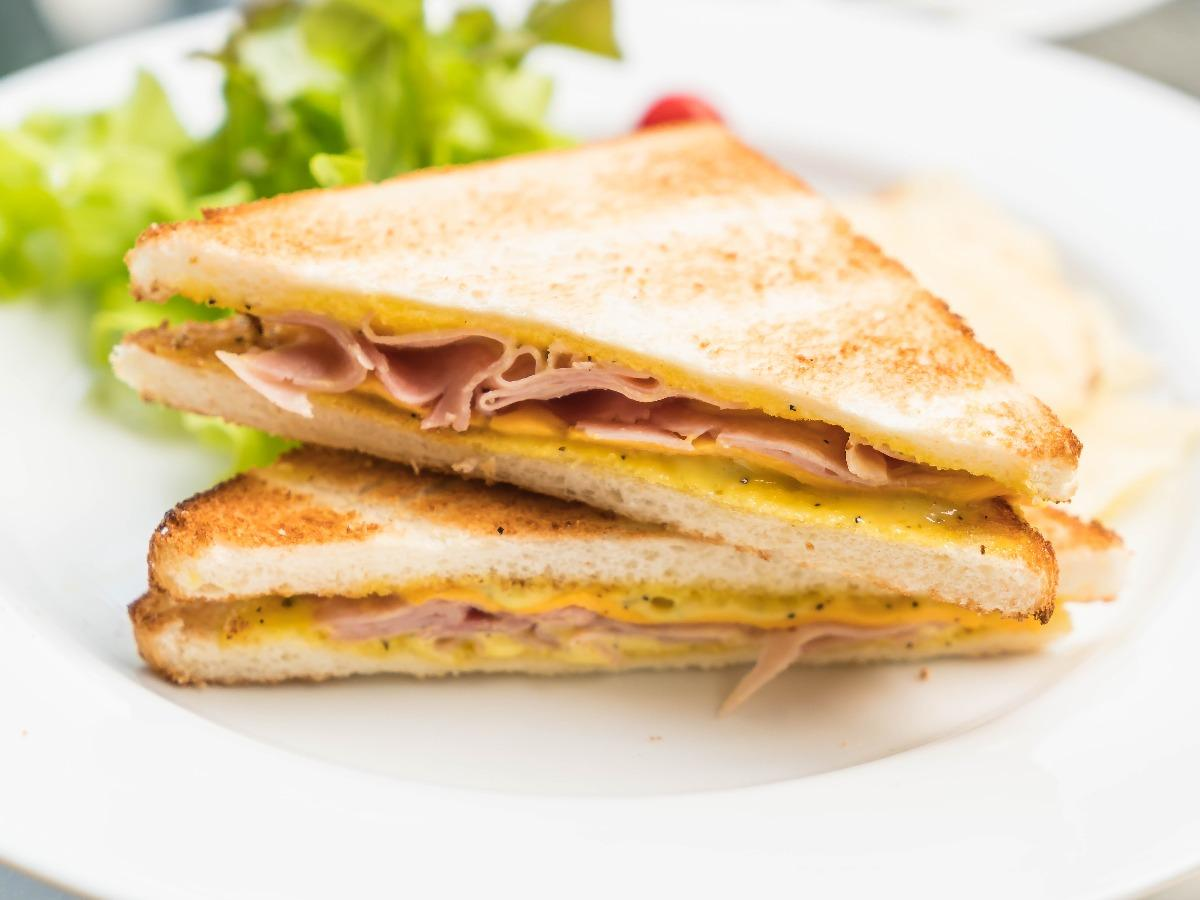
\includegraphics[height=1.5in]{images/hamcheese.jpg}
\end{center}

\textcolor{\secCol}{\section*{Ingredients}}\fontsize{12}{12}\selectfont\textcolor{\txtCol}{\textbf{
\begin{multicols}{2}
\begin{enumerate}
\item Ham
\item Cheese
\item 2 slices of bread
\item INGREDIENT
\item INGREDIENT
\item INGREDIENT
\item INGREDIENT
\item INGREDIENT
\item INGREDIENT
\\
\end{enumerate}
\end{multicols}
}}

\textcolor{\secCol}{\section*{Instructions}}\fontsize{12}{12}\selectfont\textcolor{\txtCol}{\textbf{
\begin{multicols}{2}
\begin{enumerate}
\item Put the peanut butter on a slice of bread
\item Put the jelly on the piece of bread
\item Put the 2 bread slices together
\item INSTRUCTIONS
\item INSTRUCTIONS
\item INSTRUCTIONS
\item INSTRUCTIONS
\item INSTRUCTIONS
\item INSTRUCTIONS
\\
\end{enumerate}
\end{multicols}
}}

\textcolor{\secCol}{\section*{Cultural Context}}\fontsize{14}{14}\selectfont
\noindent\textcolor{\txtCol}{
Ham and cheese Sandwiches are an essential part of any traditional suburban American household.
You can also use turkey.
\\
}

